%! Aldo Luna, Alexandra Mazzetti, Carlos Aznarán, Edward Canales
%! Universidad Nacional de Ingeniería
%! Facultad de Ciencias
%! Lima, Perú
%! Uso:
%! $ sudo pacman -Syu texlive-most zathura # dependencias, visor
%! $ arara primera
%! $ zathura primera.pdf
%! Ver https://wiki.archlinux.org/title/TeX_Live
% arara: clean: {
% arara: --> extensions:
% arara: --> ['aux','log','nav',
% arara: --> 'out','snm','toc','pytxcode','pdf']
% arara: --> }
% arara: lualatex: {
% arara: --> shell: yes,
% arara: --> draft: yes,
% arara: --> interaction: batchmode
% arara: --> }
% arara: biber
%! arara: pythontex
% arara: lualatex: {
% arara: --> shell: yes,
% arara: --> draft: yes,
% arara: --> interaction: batchmode
% arara: --> }
% arara: lualatex: {
% arara: --> shell: yes,
% arara: --> synctex: yes,
% arara: --> interaction: batchmode
% arara: --> }
% arara: clean: {
% arara: --> extensions:
% arara: --> ['aux','log','nav',
% arara: --> 'out','snm','toc','pytxcode']
% arara: --> }
\PassOptionsToPackage{svgnames}{xcolor}
\documentclass[
	spanish,
	8pt,
	utf8,
	xcolor=table,
	handout,
	aspectratio=169,
	professionalfonts,
	% notheorems,
	mathserif,
	leqno,
	% t
]{beamer}
\setbeamersize{text margin left=5pt,text margin right=5pt}
\usepackage[spanish,es-sloppy]{babel}
\spanishdatedel\decimalpoint
\usepackage{mathtools}
\usepackage{nicematrix}
\usepackage{systeme}
\usepackage{minted}
\usepackage{enumerate}
\usepackage{multicol}
% \usepackage{pythontex}
\usepackage[
	citestyle=numeric,
	style=apa,
	backend=biber,
	defernumbers=true,
	sorting=ynt,
	maxcitenames=4
]{biblatex}
\addbibresource{references.bib}

\newcolumntype{x}[1]{>{\centering\arraybackslash\hspace{0pt}}p{#1}}

\newcounter{savedenum}
\newcommand*{\saveenum}{\setcounter{savedenum}{\theenumi}}
\newcommand*{\resume}{\setcounter{enumi}{\thesavedenum}}

\setbeamertemplate{navigation symbols}{}
\setbeamertemplate{footline}{}
\setbeamertemplate{headline}{}

% https://tex.stackexchange.com/questions/68080/beamer-bibliography-icon
\setbeamertemplate{bibliography item}{%
	\ifboolexpr{ test {\ifentrytype{book}} or test {\ifentrytype{mvbook}}
		or test {\ifentrytype{collection}} or test {\ifentrytype{mvcollection}}
		or test {\ifentrytype{reference}} or test {\ifentrytype{mvreference}} }
	{\setbeamertemplate{bibliography item}[book]}
	{\ifentrytype{online}
		{\setbeamertemplate{bibliography item}[online]}
		{\setbeamertemplate{bibliography item}[article]}}%
	\usebeamertemplate{bibliography item}}

\defbibenvironment{bibliography}
{\list{}
	{\settowidth{\labelwidth}{\usebeamertemplate{bibliography item}}%
		\setlength{\leftmargin}{\labelwidth}%
		\setlength{\labelsep}{\biblabelsep}%
		\addtolength{\leftmargin}{\labelsep}%
		\setlength{\itemsep}{\bibitemsep}%
		\setlength{\parsep}{\bibparsep}}}
{\endlist}
{\item}

\title{
	\huge\sffamily
	Segunda Práctica Dirigida\quad Grupo N$^{\circ}$~1
}

\subtitle{
	\large\scshape
	Análisis y Modelamiento Numérico I\quad CM4F1 B\\[.5\baselineskip]
		\normalsize\normalfont
		Profesor Jonathan Munguia La Cotera
}

\author{
	Aldo Luna Bueno\quad\and\quad
	Alexandra Gutierrez Mazzetti\quad\and\quad
	Carlos Aznarán Laos\quad\and\quad
	Edward Canales Yarin
}

\institute{\large
	Facultad de Ciencias \and
	Universidad Nacional de Ingeniería
}
\date{12 de octubre del 2022}

\begin{document}

\frame{\titlepage}

% \begin{frame}
% 	\begin{theorem}[La regla de la cadena]
% 		Suponga que \alert{$f$ es diferenciable} en un punto interior
% 		$x_{0}$ de su dominio, y \alert{$g$ es diferenciable} en
% 		$f\left(x_{0}\right)$, un punto interior de su dominio.
% 		Entonces, \alert{$g\circ f$ es diferenciable} en $x_{0}$, y
% 		\begin{equation*}
% 			\boxed{
% 				{\left(g\circ f\right)}^{\prime}\left(x_{0}\right)=
% 				\left(g^{\prime}\circ f\right)\left(x_{0}\right)\cdot
% 				f^{\prime}\left(x_{0}\right)=
% 				g^{\prime}\left(f\left(x_{0}\right)\right)\cdot
% 				f^{\prime}\left(x_{0}\right).
% 			}
% 		\end{equation*}
% 	\end{theorem}

% 	\begin{proof}
% 		Suponga que $f$ es diferenciable en un punto interior $x_{0}$ de
% 		su dominio, y $g$ es diferenciable en $f\left(x_{0}\right)$, un
% 		punto interior de su dominio.
% 		Defina la función $h\colon\mathcal{D}\left(g\right)\to\mathbb{R}$
% 		por
% 		\begin{equation*}
% 			h\left(u\right)=
% 			\begin{cases}
% 				\dfrac{
% 					g\left(u\right)-g\left(f\left(x_{0}\right)\right)
% 				}{
% 					u-f\left(x_{0}\right)
% 				}
% 				 & \text{si }u\neq f\left(x_{0}\right); \\
% 				g^{\prime}\left(f\left(x_{0}\right)\right)
% 				 & \text{si }u=f\left(x_{0}\right).
% 			\end{cases}
% 		\end{equation*}
% 		Entonces, $h$ es continua en $f\left(x_{0}\right)$, ya que
% 		\begin{align*}
% 			\lim\limits_{u\to f\left(x_{0}\right)}
% 			h
% 			\left(u\right)                   & =
% 			\lim\limits_{u\to f\left(x_{0}\right)}
% 			\frac{
% 				g\left(u\right)-
% 				g\left(f\left(x_{0}\right)\right)
% 			}{
% 				u-
% 				f\left(x_{0}\right)
% 			}                                &              & \qquad
% 			u\neq f\left(x_{0}\right)
% 			\text{ cuando }u\to f\left(x_{0}\right)                  \\
% 			                                 & = g^{\prime}
% 			\left(f\left(x_{0}\right)\right) &              & \qquad
% 			\text{por definición de la derivada}                     \\
% 			                                 & = h
% 			\left(f\left(x_{0}\right)\right) &              & \qquad
% 			\text{por definición de $h$}
% 		\end{align*}
% 		Ahora, $\forall u\in\mathcal{D}\left(g\right)$, incluso si
% 		$u=f\left(x_{0}\right)$, la definición de $h\left(u\right)$
% 		resulta
% 		\begin{math}
% 			g\left(u\right)-g\left(f\left(x_{0}\right)\right)=
% 			h\left(u\right)
% 			\left(u-f\left(x_{0}\right)\right)
% 		\end{math}.
% 	\end{proof}
% \end{frame}

% \begin{frame}
% 	\begin{proof}
% 		Por lo tanto, para todo $x$ en una vecindad reducida de $x_{0}$,
% 		\begin{align*}
% 			\frac{
% 			\left(g\circ f\right)\left(x\right)-
% 			\left(g\circ f\right)\left(x_{0}\right)
% 			}{
% 			x-x_{0}
% 			} & =
% 			\frac{
% 			g\left(f\left(x\right)\right)-
% 			g\left(f\left(x_{0}\right)\right)
% 			}{
% 			x-x_{0}
% 			}                                  \\
% 			  & =\frac{
% 			h
% 			\left(f\left(x\right)\right)
% 			\left(
% 			f\left(x\right)-
% 			f\left(x_{0}\right)
% 			\right)
% 			}{
% 			x-x_{0}
% 			}                                  \\
% 			  & =h\left(f\left(x\right)\right)
% 			\frac{
% 			f\left(x\right)-f\left(x_{0}\right)
% 			}{
% 			x-x_{0}
% 			}.
% 			\shortintertext{Así,}
% 			\lim\limits_{x\to x_{0}}
% 			\frac{
% 			\left(g\circ f\right)\left(x\right)-
% 			\left(g\circ f\right)\left(x_{0}\right)
% 			}{
% 			x-x_{0}
% 			}
% 			  & =
% 			\lim\limits_{x\to x_{0}}
% 			h
% 			\left(f\left(x\right)\right)
% 			\lim\limits_{x\to x_{0}}
% 			\frac{
% 			f\left(x\right)-f\left(x_{0}\right)
% 			}{
% 			x-x_{0}
% 			}                                  \\
% 			  & =
% 			h
% 			\left(f\left(x_{0}\right)\right)
% 			f^{\prime}\left(x_{0}\right)       \\
% 			  & = g^{\prime}
% 			\left(f\left(x_{0}\right)\right)
% 			f^{\prime}\left(x_{0}\right).
% 		\end{align*}
% 	\end{proof}
% \end{frame}

% \begin{frame}

% 	\begin{definition}[Función inversa]
% 		Suponga $f\colon A\to B$.
% 		Si $\exists$ función $g\colon B\to A$ tal que $g\circ f=i_{A}$
% 		y $f\circ g=i_{B}$, entonces decimos que $f$ es
% 		\alert{invertible}, y decimos que la función $g$
% 		es la \alert{función inversa} de $f$.
% 		En símbolos, $g=f^{-1}$.
% 	\end{definition}

% 	\

% 	\begin{theorem}
% 		Una función $f\colon A\to B$ es \alert{inversible} sii $f$ es 1-1
% 		y sobre $B$ (esto es, $f$ es una correspondencia 1-1).
% 		Más aún, si $g=f^{-1}$, entonces $f=g^{-1}$.
% 	\end{theorem}

% 	\

% 	\begin{proof}
% 		\begin{itemize}
% 			\item[$\left(\Rightarrow\right)$]

% 				Suponga que $f\colon A\to B$ es inversible.
% 				Entonces, $\exists$ función $g\colon B\to A$ tal que
% 				$g\circ f=i_{A}$ y $f\circ g=i_{B}$.
% 				Dado que $i_{A}$ es 1-1, decimos que $f$ es 1-1.
% 				Dado que $i_{B}$ sobre $B$, decimos que $f$ es sobre $B$.

% 				\

% 			\item[$\left(\Leftarrow\right)$]

% 				Suponga que $f\colon A\to B$ es 1-1 y sobre $B$.
% 				Sea $b\in B$.
% 				Dado que $f$ es sobre $B$, $\exists a\in A$ tal que
% 				$f\left(a\right)=b$.
% 				Más aún, dado que $f$ es 1-1, no existe más que tal $a$.
% 				Defina

% 				\begin{equation*}
% 					g\left(b\right)\coloneqq a.
% 				\end{equation*}

% 				Entonces, $\forall a\in A$,
% 				\begin{math}
% 					\left(g\circ f\right)\left(a\right)=
% 					g\left(f\left(a\right)\right)=
% 					g\left(b\right)=
% 					a=
% 					i_{A}\left(a\right)
% 				\end{math}.
% 				También, $\forall b\in B$,
% 				\begin{math}
% 					\left(f\circ g\right)\left(b\right)=
% 					f\left(g\left(b\right)\right)=
% 					f\left(a\right)=
% 					b=
% 					i_{B}\left(b\right)
% 				\end{math}.
% 				Esto es, $g\circ f=i_{A}$ y $f\circ g=i_{B}$.
% 		\end{itemize}
% 	\end{proof}
% \end{frame}


% \begin{frame}
% 	\begin{theorem}[Teorema de la función inversa para funciones monótonas continuas]
% 		Suponga que $I$ es un intervalo no vacío, y
% 		$f\colon I\to\mathbb{R}$ es
% 		\alert{continua y estrictamente monótona}.
% 		Entonces, $f^{-1}\colon f\left(I\right)\to I$ es
% 		\alert{continua y estrictamente monótona} en el mismo sentido.
% 	\end{theorem}

% 	\

% 	\begin{proof}
% 		Suponga que $I$ es un intervalo no vacío, y
% 		$f\colon I\to\mathbb{R}$ es continua y estrictamente monótona.
% 		Entonces, $f\colon I\to f\left(I\right)$ es una correspondencia
% 		1-1, y así tiene una inversa,
% 		$f^{-1}\colon f\left(I\right)\to I$, que es también 1-1 y sobre.
% 		Luego, $f^{-1}$ es estrictamente creciente en $f\left(I\right)$.
% 		Así, $f^{-1}\colon f\left(I\right)\to I$ es continua en
% 		$f\left(I\right)$.
% 	\end{proof}

% 	\

% 	\begin{theorem}[Criterio de sucesiones para la diferenciabilidad]
% 		Suponga que $f\colon\mathcal{D}\left(f\right)\to\mathbb{R}$ y
% 		$x_{0}$ es un punto interior de $\mathcal{D}\left(f\right)$.
% 		Entonces, \alert{$f$ es diferenciable} en $x_{0}$ con la derivada
% 		$f^{\prime}\left(x_{0}\right)$ sii
% 		$\forall$ sucesión $\left\{x_{n}\right\}$ en
% 		$\mathcal{D}\left(f\right)\setminus\left\{x_{0}\right\}$
% 		tal que
% 		\begin{equation*}
% 			\boxed{
% 			x_{n}\to
% 			x_{0},\quad
% 			\frac{f\left(x_{n}\right)-f\left(x_{0}\right)}{x_{n}-x_{0}}\to
% 			f^{\prime}\left(x_{0}\right).
% 			}
% 		\end{equation*}
% 	\end{theorem}
% \end{frame}

% \begin{frame}
% 	\begin{theorem}[Teorema de la función inversa para funciones diferenciables]
% 		Suponga que \alert{$f$ es 1-1 y continua} sobre un intervalo
% 		abierto $I$.
% 		Si \alert{$f$ es diferenciable} en un punto $x_{0}\in I$ y
% 		$f^{\prime}\left(x_{0}\right)\neq0$, entonces
% 		\alert{$f^{-1}$ es diferenciable} en $f\left(x_{0}\right)$,
% 		y
% 		\begin{math}
% 			{\left(f^{-1}\right)}^{\prime}\left(f\left(x_{0}\right)\right)=
% 			\dfrac{1}{f^{\prime}\left(x_{0}\right)}
% 		\end{math}.
% 	\end{theorem}

% 	\

% 	\begin{proof}
% 		Suponga que $f$ es 1-1 y continua en un intervalo abierto $I$,
% 		diferenciable en un punto $x_{0}\in I$,
% 		y $f^{\prime}\left(x_{0}\right)\neq0$.
% 		Sea $y_{0}=f\left(x_{0}\right)$.
% 		Usaremos el criterio de sucesiones para la diferenciabilidad.
% 		Sea $\left\{y_{n}\right\}$ una sucesión en
% 		$f\left(I\right)\setminus\left\{y_{0}\right\}$ convergiendo a
% 		$y_{0}$.
% 		Entonces, $\forall n\in\mathbb{N}$, sea
% 		$x_{n}=f^{-1}\left(y_{n}\right)$; es decir,
% 		$y_{n}=f\left(x_{n}\right)$.
% 		Note que $\forall n\in\mathbb{N}$, sea $x_{n}\neq x_{0}$.
% 		Entonces,

% 		\begin{align*}
% 			\lim\limits_{n\to\infty}
% 			\frac{
% 			f^{-1}\left(y_{n}\right)-
% 			f^{-1}\left(y_{0}\right)
% 			}{
% 			y_{n}-y_{0}
% 			} & =
% 			\lim\limits_{n\to\infty}
% 			\frac{
% 			x_{n}-x_{0}
% 			}{
% 			f\left(x_{n}\right)-
% 			f\left(x_{0}\right)
% 			}                                                       \\
% 			  & =
% 			\lim\limits_{n\to\infty}
% 			\left(
% 			\frac{1}{
% 				\frac{
% 					f\left(x_{n}\right)-f\left(x_{0}\right)
% 				}{
% 					x_{n}-x_{0}
% 				}
% 			}
% 			\right)                                                 \\
% 			  & =
% 			\frac{1}{
% 			\lim\limits_{n\to\infty}
% 			\frac{
% 			f\left(x_{n}\right)-f\left(x_{0}\right)
% 			}{x_{n}-x_{0}}
% 			}\qquad\text{por el álgebra de límites para sucesiones} \\
% 			  & =
% 			\frac{1}{
% 				f^{\prime}\left(x_{0}\right)
% 			}\qquad
% 			\text{
% 				ya que $f$ es diferenciable en $x_{0}$, y
% 				$f^{\prime}\left(x_{0}\right)\neq0$
% 			}.
% 		\end{align*}

% 		Por el criterio de sucesiones para derivadas,
% 		\begin{math}
% 			{\left(f^{-1}\right)}^{\prime}
% 			\left(f\left(x_{0}\right)\right)=
% 			\dfrac{1}{f^{\prime}\left(x_{0}\right)}
% 		\end{math}.
% 	\end{proof}
% \end{frame}

\begin{frame}
	\frametitle{Pregunta N$^{\circ}$~2}

	Suponga que $f$ y $g$ son funciones de valor real que
	tienen números de condición $\kappa_{f}$ y $\kappa_{g}$,
	respectivamente.
	Defina una nueva función
	\begin{math}
		h\left(x\right)=
		\left(f\circ g\right)
		\left(x\right)
	\end{math}.
	Muestre que para $x$ en el dominio de $h$, el número de
	condición de $h$ satisface
	\begin{equation*}
		\boxed{
			\kappa_{h}\left(x\right)=
			\kappa_{f}\left(g\left(x\right)\right)\cdot
			\kappa_{g}\left(x\right).
		}
	\end{equation*}

	\

	\begin{proof}
		% \begin{enumerate}[a)]
		% 	\item

		Si $f$ y $g$ son funciones diferenciables con
		$g\left(x\right)\neq0$, entonces por la regla de cadena tenemos
		\begin{math}
			h^{\prime}
			\left(x\right)=
			f^{\prime}
			\left(g\left(x\right)\right)
			g^{\prime}\left(x\right).
		\end{math}

		Por definición, el número de condición del problema $h$ en
		$x$ es

		\begin{equation*}
			\kappa_{h}
			\left(x\right)=
			\left|
			\frac{
				xh^{\prime}
				\left(
				x
				\right)
			}{
				h
				\left(
				x
				\right)
			}
			\right|=
			\left|
			\frac{
				xf^{\prime}
				\left(
				g\left(x\right)
				\right)
				g^{\prime}
				\left(
				x
				\right)
			}{
				f\left(
				g\left(x\right)
				\right)
			}
			\right|=
			\left|
			\frac{
				xf^{\prime}
				\left(
				g\left(x\right)
				\right)
				g^{\prime}
				\left(x\right)
				\alert{g\left(x\right)}
			}{
				f\left(g\left(x\right)\right)
				\alert{g\left(x\right)}
			}
			\right|=
			\left|
			\frac{
				\alert{g\left(x\right)}
				f^{\prime}
				\left(g\left(x\right)\right)
			}{
				f\left(
				g\left(x\right)
				\right)
			}
			\right|
			\left|
			\frac{
				xg^{\prime}\left(x\right)
			}{
				\alert{g\left(x\right)}
			}
			\right|=
			\kappa_{f}\left(g\left(x\right)\right)\cdot
			\kappa_{g}\left(x\right)
			.
		\end{equation*}

		% \item

		%       Por definición, el número de condición de $h$ es
		%       \begin{equation*}
		% 	      \kappa_{h}\left(x\right)=
		% 	      \lim\limits_{\delta\to0}
		% 	      \sup\limits_{\left|j\right|<\delta}
		% 	      \left|
		% 	      \frac{
		% 		      \frac{
		% 			      h\left(x+j\right)-h\left(x\right)
		% 		      }{
		% 			      h\left(x\right)
		% 		      }
		% 	      }{\frac{j}{x}}
		% 	      \right|
		% 	      =
		% 	      \lim\limits_{\delta\to0}
		% 	      \sup\limits_{\left|j\right|<\delta}
		% 	      \left|
		% 	      \frac{
		% 		      \frac{
		% 			      f\left(g\left(x\right)+j\right)-
		% 			      f\left(g\left(x\right)\right)
		% 		      }{
		% 			      f\left(g\left(x\right)\right)
		% 		      }
		% 	      }{
		% 		      \frac{j}{g\left(x\right)}
		% 	      }
		% 	      \right|
		% 	      \lim\limits_{\delta\to0}
		% 	      \sup\limits_{\left|j\right|<\delta}
		% 	      \left|
		% 	      \frac{
		% 		      \frac{
		% 			      g\left(x+j\right)-g\left(x\right)
		% 		      }{
		% 			      g\left(x\right)
		% 		      }
		% 	      }{\frac{j}{x}}
		% 	      \right|
		% 	      =
		% 	      \kappa_{f}
		% 	      \left(g\left(x\right)\right)\cdot
		% 	      \kappa_{g}
		% 	      \left(x\right).
		%       \end{equation*}
		% \end{enumerate}
	\end{proof}
\end{frame}

\begin{frame}

	\begin{enumerate}\setcounter{enumi}{3}
		\item

		      Suponga que $f$ es una función con número de condición
		      $\kappa_{f}$, y que $f^{-1}$ es su función inversa.
		      Muestre que el número de condición de $f^{-1}$ satisface

		      \begin{equation*}
			      \boxed{
				      \kappa_{f^{-1}}\left(x\right)=
				      \frac{1}{\kappa_{f}\left(f^{-1}\left(x\right)\right)},
			      }
		      \end{equation*}

		      siempre que el denominador sea distinto de cero.

	\end{enumerate}

	\begin{solution}
		De la pregunta N$^{\circ}$~2, sabemos que
		\begin{math}
			\kappa_{h}\left(x\right)=
			\kappa_{f}\left(g\left(x\right)\right)\cdot
			\kappa_{g}\left(x\right)
		\end{math}.
		Aplicando la identidad anterior para las funciones $f=f$ y
		$g=f^{-1}$ con $g\left(x\right)\neq0$, es decir, $h=f\circ g=x$,
		tenemos
		\begin{equation*}
			\kappa_{x}\left(x\right)=
			\left|\frac{x\cdot x^{\prime}}{x}\right|=
			1=
			\kappa_{f}\left(f^{-1}\left(x\right)\right)\cdot
			\kappa_{f^{-1}}\left(x\right)\implies
			\frac{1}{\kappa_{f}\left(f^{-1}\left(x\right)\right)}=
			\kappa_{f^{-1}}\left(x\right).
		\end{equation*}
	\end{solution}
\end{frame}

\begin{frame}
	\begin{definition}[Símbolos de Landau]
		Sean $x_{n},y_{n}\colon\mathbb{N}\to\mathbb{R}$ dos sucesiones.

		\begin{enumerate}[a)]
			\item

			      Decimos que $x_{n}$ es ``\alert{$O$ grande}'' de $y_{n}$
			      sii existen constantes $C>0$ y $n_{0}\in\mathbb{N}$
			      tales que
			      \begin{equation*}
				      \left|
				      x_{n}
				      \right|\leq
				      C
				      \left|
				      y_{n}
				      \right|\quad
				      \forall n\geq n_{0}.
			      \end{equation*}
			      Escribimos
			      \begin{math}
				      x_{n}\in
				      O\left(y_{n}\right)
			      \end{math}
			      o con abuso de notación como
			      \begin{math}
				      x_{n}=
				      O\left(y_{n}\right)
			      \end{math}.

			      \

			\item

			      Decimos que $x_{n}$ es ``\alert{$o$ pequeña}'' de $y_{n}$
			      sii existe una sucesión
			      \begin{math}
				      \left\{\epsilon_{n}\right\}_{n\in\mathbb{N}}\subset
				      \mathbb{R}^{+}_{0}
			      \end{math}
			      que converge a $0$ tal que
			      \begin{equation*}
				      \left|
				      x_{n}
				      \right|\leq
				      \epsilon_{n}
				      \left|
				      y_{n}
				      \right|\quad
				      \forall n\in\mathbb{N}.
			      \end{equation*}
			      Escribimos
			      \begin{math}
				      x_{n}\in
				      o\left(y_{n}\right)
			      \end{math}
			      o con abuso de notación como
			      \begin{math}
				      x_{n}=
				      o\left(y_{n}\right)
			      \end{math}.
		\end{enumerate}
	\end{definition}
	% \begin{alertblock}{Propiedades cuando $x\to x_{0}$}
	% 	\begin{multicols}{2}

	% 		\begin{enumerate}[i)]
	% 			\item

	% 			      \begin{math}
	% 				      f\left(x\right)=
	% 				      O\left(f\left(x\right)\right)
	% 			      \end{math}.

	% 			\item

	% 			      \begin{math}
	% 				      f\left(x\right)=
	% 				      o\left(g\left(x\right)\right)\implies
	% 				      f\left(x\right)=
	% 				      O\left(g\left(x\right)\right)
	% 			      \end{math}.

	% 			\item

	% 			      \begin{math}
	% 				      \exists
	% 				      K\in\mathbb{R},
	% 				      f\left(x\right)=K\cdot
	% 				      O\left(g\left(x\right)\right)
	% 				      \implies
	% 				      f\left(x\right)=O\left(g\left(x\right)\right)
	% 			      \end{math}.

	% 			\item

	% 			      \begin{math}
	% 				      f(x)=O\left(g_1(x)\right),
	% 				      g_{1}\left(x\right)=
	% 				      O\left(g_2(x)\right)\implies
	% 				      f(x)=O\left(g_2(x)\right)
	% 			      \end{math}.

	% 			\item

	% 			      \begin{math}
	% 				      f_{1}\left(x\right)=
	% 				      O\left(g_{1}\left(x\right)\right),
	% 				      f_{2}\left(x\right)=
	% 				      O\left(g_{2}\left(x\right)\right)\implies
	% 				      f_{1}\left(x\right)\cdot
	% 				      f_{2}\left(x\right)=
	% 				      O\left(g_{1}\left(x\right)\cdot
	% 				      g_{2}\left(x\right)\right)
	% 			      \end{math}.

	% 			\item

	% \begin{math}
	%   f\left(x\right)=
	%   O\left(
	% 		g_{1}\left(x\right)g_{2}\left(x\right)
	% 		\right)\implies
	%   f\left(x\right)=g_{1}\left(x\right)\cdot
	%   O\left(g_{2}\left(x\right)\right)
	% \end{math}.
	% 		\end{enumerate}
	% 	\end{multicols}
	% 	% Los análogos de las propiedades (iii) - (vi) también se cumplen
	% 	% para el símbolo ``$o$''.
	% \end{alertblock}
	\begin{theorem}
		Sea $a_{n}$ una sucesión de números reales o complejos.
		Las siguientes proposiciones son equivalentes:
		\begin{multicols}{2}
			\begin{enumerate}[a)]
				\item

				      $a_{n}$ es acotada.

				\item

				      $a_{n}=O\left(1\right)$.
			\end{enumerate}
		\end{multicols}
	\end{theorem}

	\begin{proof}
		\begin{math}
			a_{n}\text{ es acotada}
			\iff\exists k\in\mathbb{R},
			\left|a_{n}\right|\leq k
			\iff\exists k\in\mathbb{R},
			\left|a_{n}\right|\leq
			k\cdot
			\left|1\right|
			\iff a_{n}=
			O\left(1\right).
		\end{math}
	\end{proof}
\end{frame}
% \begin{frame}[fragile]
% 	\printpythontex
% \end{frame}

\begin{frame}
	\begin{enumerate}\setcounter{enumi}{5}
		\item
		      Determine el Landau de las siguientes funciones

		      \begin{multicols}{4}
			      \begin{enumerate}[a)]

				      \item

				            \begin{math}
					            \dfrac{1}{n^{2}}.
				            \end{math}

				      \item

				            \begin{math}
					            \cos\left(n\right).
				            \end{math}


				      \item

				            \begin{math}
					            \sin\left(\dfrac{x}{n}\right).
				            \end{math}

				      \item

				            \begin{math}
					            \sqrt{n+1}-\sqrt{n}.
				            \end{math}
			      \end{enumerate}
		      \end{multicols}

	\end{enumerate}

	\begin{solution}
		\begin{enumerate}[a)]

			\item

			      \begin{math}
				      \dfrac{1}{n^{2}}=
				      O\left(\frac{1}{n}\right)
			      \end{math}
			      porque existen $C=\alert{1}>0$, $n=1\in\mathbb{N}$ tales
			      que

			      \begin{equation*}
				      \left|
				      \frac{1}{n^{2}}
				      \right|\leq
				      \alert{1}\left|
				      \frac{1}{n}
				      \right|\quad
				      \forall n\geq 1.
			      \end{equation*}

			\item

			      \begin{math}
				      \cos\left(n\right)=
				      O\left(1\right)
			      \end{math}
			      porque existen $C=\alert{1}>0$, $n=1\in\mathbb{N}$ tales
			      que

			      \begin{equation*}
				      \left|
				      \cos\left(n\right)
				      \right|\leq
				      \alert{1}\left|
				      1
				      \right|\quad
				      \forall n\geq 1.
			      \end{equation*}

			\item

			      \begin{math}
				      \sin\left(\dfrac{x}{n}\right)=
				      O\left(1\right)
			      \end{math}
			      porque existen $C=\alert{1}>0$, $n=1\in\mathbb{N}$ tales
			      que

			      \begin{equation*}
				      \left|
				      \sin\left(\frac{x}{n}\right)
				      \right|\leq
				      \alert{1}\left|
				      1
				      \right|\quad
				      \forall n\geq 1.
			      \end{equation*}

			\item

			      \begin{math}
				      \sqrt{n+1}-\sqrt{n}=
				      O\left(\frac{1}{\sqrt{n}}\right)
			      \end{math}
			      porque existen $C=\alert{\dfrac{1}{2}}>0$,
			      $n=1\in\mathbb{N}$ tales que

			      \begin{equation*}
				      \left|
				      \sqrt{n+1}-\sqrt{n}
				      \right|=
				      \left|
				      \left(\sqrt{n+1}-\sqrt{n}\right)\cdot
				      \alert{\frac{\sqrt{n+1}+\sqrt{n}}{\sqrt{n+1}+\sqrt{n}}}
				      \right|=
				      \left|
				      \frac{n+1-n}{\sqrt{n+1}+\sqrt{n}}
				      \right|
				      \leq
				      \left|
				      \frac{1}{\sqrt{n}+\sqrt{n}}
				      \right|=
				      \alert{\dfrac{1}{2}}
				      \left|
				      \frac{1}{\sqrt{n}}
				      \right|
				      \quad
				      \forall n\geq 1.
			      \end{equation*}
		\end{enumerate}
	\end{solution}
\end{frame}

\begin{frame}
	\begin{definition}[Matriz ortogonal]
		Una matriz $A\in\mathbb{R}^{n\times n}$ es \alert{ortogonal} sii
		$A^{t}A=AA^{t}=I_{n}$.
	\end{definition}

	\

	\begin{example}
		La matriz
		\begin{equation*}
			A=
			\begin{bNiceMatrix}
				\cos \alpha  & \sin \alpha \\
				-\sin \alpha & \cos \alpha
			\end{bNiceMatrix}
		\end{equation*}
		es ortogonal.
	\end{example}

	\


	\begin{theorem}
		Si $U$ es una matriz ortogonal, entonces
		\begin{math}
			{\left\|Ux\right\|}_{2}=
				{\left\|x\right\|}_{2}
		\end{math}
		(esto es, la longitud de cualquier vector es invariante bajo la
		multiplicación por $U$).
	\end{theorem}

	\

	\begin{proof}
		Si $U$ es ortogonal tenemos
		\begin{equation*}
			{\left\|Ux\right\|}^{2}_{2}=
				{\left(Ux\right)}^{t}
			Ux=
			x^{t}U^{t}Ux=
				{\left\|x\right\|}^{2}_{2}
		\end{equation*}
		porque $U^{t}U=I_{n}$.
		Por lo tanto,
		\begin{math}
			{\left\|Ux\right\|}_{2}=
				{\left\|x\right\|}_{2}
		\end{math}.
	\end{proof}
\end{frame}

\begin{frame}
	\begin{alertblock}{Propiedades}
		Sea $U$ una matriz ortogonal.

		\

		\begin{enumerate}[a)]
			\item

			      La inversa de una matriz ortogonal es $U^{-1}=U^{t}$.

			      \

			\item

			      \begin{math}
				      \det\left(U\right)=\pm1
			      \end{math}.

			      \

			\item

			      La norma de Frobenius
			      \begin{math}
				      {\left\|\cdot\right\|}_{F}
			      \end{math}
			      es invariante.

			      \begin{equation*}
				      {\left\|UA\right\|}_{F}=
				      \sqrt{
					      \operatorname{traza}
					      \left(
					      {\left(UA\right)}^{t}
					      UA
					      \right)}=
				      \sqrt{
					      \operatorname{traza}
					      \left(
					      A^{t}U^{t}UA
					      \right)}=
				      \sqrt{
					      \operatorname{traza}
					      \left(
					      A^{t}A
					      \right)
				      }=
				      {\left\|A\right\|}_{F}.
			      \end{equation*}

			      \

			\item

			      La norma
			      \begin{math}
				      {\left|\left\|\cdot\right\|\right|}_{2}
			      \end{math}
			      es invariante.

			      \begin{equation*}
				      {\left|\left\|UA\right\|\right|}_{2}=
				      \max
				      \left\{
				      {\left\|\left(UA\right)x\right\|}_{2}:
				      {\left\|x\right\|}_{2}=
				      1
				      \right\}=
				      \max
				      \left\{
				      \|U(Ax)\|_{2}:
				      {\left\|x\right\|}_{2}=
				      1
				      \right\}
				      =\max
				      \left\{
				      {\left\|Ax\right\|}_{2}:
				      {\left\|x\right\|}_{2}=1
				      \right\}
				      =
				      {\left\|A\right\|}_{2}.
			      \end{equation*}
		\end{enumerate}
	\end{alertblock}
\end{frame}

\begin{frame}
	\begin{alertblock}{Algunos resultados}

		\begin{enumerate}[(a)]
			% \item

			%       Si $a<b$ y $c>0$, entonces $ac<bc$
			%       (consistencia multiplicativa).

			\item

			      Si $A$ y $B$ son inversibles, entonces

			      \begin{align*}
				      \left(AB\right){\left(AB\right)}^{-1}
				       & =I_{n}         \\
				      \left(\alert{A^{-1}A}B\right)\left(AB\right)^{-1}
				       & =A^{-1}I_{n}   \\
				      \left(I_{n}B\right){\left(AB\right)}^{-1}
				       & =A^{-1}        \\
				      B{\left(AB\right)}^{-1}
				       & =A^{-1}        \\
				      \alert{B^{-1}B}{\left(AB\right)}^{-1}
				       & =B^{-1}A^{-1}  \\
				      I_{n}{\left(AB\right)}^{-1}
				       & =B^{-1}A^{-1}  \\
				      {\left(AB\right)}^{-1}
				       & =B^{-1}A^{-1}.
			      \end{align*}

			\item

			      Si $A\in\mathbb{R}^{m\times n}$ y
			      \begin{math}
				      \rho
				      \left(H\right)=
				      \max
				      \left\{
				      \left|\lambda\right|: Hv=\lambda v, v\neq0
				      \right\}
			      \end{math}
			      donde $H$ es una matriz simétrica,
			      entonces la
			      \begin{align*}
				      {\left\|A\right\|}_{2}
				                              & =
				      \sup\limits_{{\left\|x\right\|}_{2}=1}
				      {\left\|Ax\right\|}_{2} &
				      \text{definición de norma matricial} \\
				                              & =
				      \sup\limits_{{\left\|x\right\|}_{2}=1}
				      \sqrt{x^{t}A^{t}Ax}     &
				      \text{ya que }
				      \sqrt{\left\langle\cdot,\cdot\right\rangle}=
				      \left\|\cdot\right\|                 \\
				                              & =
				      \sqrt{\rho\left(A^{t}A\right)}.
				                              &
				      \text{ya que }\sqrt{x^{t}A^{t}Ax}\leq\sqrt{\lambda_{n}}
			      \end{align*}

			\item

			      Si $A$ es una matriz ortogonal, entonces
			      $\kappa\left(A\right)=1$ porque
			      \begin{math}
				      {\left\|A\right\|}_{2}=
				      \sqrt{\rho\left(A^{t}A\right)}=
				      \sqrt{\rho\left(A^{-1}A\right)}=
				      \sqrt{\rho\left(I_{n}\right)}=
				      \sqrt{1}=1
			      \end{math}.
		\end{enumerate}
	\end{alertblock}
\end{frame}

\begin{frame}

	\begin{enumerate}\setcounter{enumi}{12}
		\item

		      Suponga que $A=UBV$ con $U$, $V$ ortogonales y $B$ no
		      singular.
		      Demuestre que
		      \begin{math}
			      \kappa\left(A\right)=
			      \kappa\left(B\right)
		      \end{math}.

	\end{enumerate}

	\begin{solution}
		$A$ es inversible porque el
		\begin{equation*}
			\det\left(A\right)=
			\det\left(UBV\right)=
			\det\left(UB\left(V\right)\right)=
			\det\left(UB\right)\det\left(V\right)=
			\underbrace{\det\left(U\right)}_{\neq0}
			\underbrace{\det\left(B\right)}_{\neq0}
			\underbrace{\det\left(V\right)}_{\neq0}\neq0,
		\end{equation*}
		porque $U$, $B$ y $V$ son matrices inversibles.

		\begin{align*}
			\shortintertext{Luego,}
			\kappa\left(A\right)                            & =
			\left\|
			U\alert{BV}
			\right\|
			\left\|
			{\left(UB\alert{V}\right)}^{-1}
			\right\|                                        &
			\text{definición del número de condición de $A$}            \\
			                                                & \leq
			\left\|
			U
			\right\|
			\left\|
			\alert{BV}
			\right\|
			\left\|
			\alert{{V}^{-1}}{\left(U\alert{B}\right)}^{-1}
			\right\|                                        &
			\left\|A\alert{B}\right\|\leq
			\left\|A\right\|\left\|\alert{B}\right\|,\quad
			{\left(A\alert{B}\right)}^{-1}=\alert{B^{-1}}A^{-1}         \\
			                                                & \leq
			\left\|U\right\|
			\left\|B\right\|
			\left\|
			\alert{V}
			\right\|
			\left\|{V}^{-1}\alert{{B}^{-1}}{U}^{-1}\right\| &
			\left\|A\alert{B}\right\|\leq
			\left\|A\right\|\left\|\alert{B}\right\|,\quad
			{\left(A\alert{B}\right)}^{-1}=\alert{B^{-1}}A^{-1}         \\
			                                                & \leq
			\left\|U\right\|
			\left\|B\right\|
			\left\|V\right\|
			\left\|{V}^{-1}\right\|
			\left\|{B}^{-1}\right\|
			\left\|{U}^{-1}\right\|                         &
			\text{aplicando dos veces }
			\left\|A\alert{B}\right\|\leq
			\left\|A\right\|\left\|\alert{B}\right\|                    \\
			                                                & =
			\left\|U\right\|
			\left\|{U}^{-1}\right\|
			\left\|V\right\|
			\left\|{V}^{-1}\right\|
			\left\|B\right\|
			\left\|{B}^{-1}\right\|                         &           \\
			                                                & =
			\kappa\left(U\right)
			\kappa\left(V\right)
			\kappa\left(B\right)                            &
			\text{definición del número de condición de $U$, $V$ y $B$} \\
			                                                & =
			1\cdot 1\cdot\kappa\left(B\right)               &
			\text{$\kappa\left(A\right)=1$ cuando $A$ es ortogonal}     \\
			                                                & =
			\kappa\left(B\right).
		\end{align*}
	\end{solution}
\end{frame}

\begin{frame}

	\begin{enumerate}\setcounter{enumi}{14}
		\item

		      Utilice la eliminación gaussiana con sustitución hacia
		      atrás y aritmética de redondeo de dos dígitos para
		      resolver los siguientes sistemas lineales.
		      No reordene las ecuaciones.
		      (La solución exacta de cada sistema es $x_{1}=-1$,
		      $x_{2}=1$, $x_{3}=3$.)

		      \begin{multicols}{2}
			      \begin{enumerate}[a)]
				      \item

				            \begin{math}
					            \systeme{
					            -x_{1}+
					            4x_{2}+
					            x_{3}=
					            8,
					            \frac{5}{3}x_{1}+
					            \frac{2}{3}x_{2}+
					            \frac{2}{3}x_{3}=
					            1,
					            2x_{1}+
					            x_{2}+
					            4x_{3}=
					            11
					            }
				            \end{math}.

				      \item


				            \begin{math}
					            \systeme{
					            4x_{1}+
					            2x_{2}-
					            x_{3}=
					            -5,
					            \frac{1}{9}x_{1}+
					            \frac{1}{9}x_{2}-
					            \frac{1}{3}x_{3}=
					            -1,
					            x_{1}+
					            4x_{2}+
					            2x_{3}=
					            9
					            }
				            \end{math}.
			      \end{enumerate}
		      \end{multicols}

	\end{enumerate}

	\begin{solution}
		Los sistemas producen la matrices aumentadas

		\begin{equation*}
			\widetilde{A}=
			\left[\begin{NiceArray}{ccc:c}
					-1          & 4           & 1           & 8  \\
					\frac{5}{3} & \frac{2}{3} & \frac{2}{3} & 1  \\
					2           & 1           & 4           & 11
				\end{NiceArray}\right],\qquad
			\widetilde{B}=
			\left[\begin{NiceArray}{ccc:c}
					4           & 2           & -1           & -5 \\
					\frac{1}{9} & \frac{1}{9} & -\frac{1}{3} & -1 \\
					1           & 4           & 2            & 9
				\end{NiceArray}\right].
		\end{equation*}

		\

		\begin{itemize}
			\item

			      Puesto que $a_{11}=-1$, realizamos
			      $\left(F_{2}+\frac{5}{3}F_{1}\right)\to\left(F_{2}\right)$
			      y $\left(F_{3}+2F_{1}\right)\to\left(F_{3}\right)$ para
			      obtener $a_{22}=a_{32}=0$.

			      \

			\item

			      Puesto que $b_{11}=4$, realizamos
			      \begin{math}
				      \left(F_{3}-\frac{1}{4}F_{1}\right)\to
				      \left(F_{3}\right)
			      \end{math}
			      y
			      \begin{math}
				      \left(F_{2}-\frac{0.11}{4}F_{1}\right)\to
				      \left(F_{2}\right)
			      \end{math}
			      para obtener
			      $b_{22}=b_{32}=0$.
		\end{itemize}
	\end{solution}
\end{frame}

\begin{frame}
	\begin{minipage}{0.35\textwidth}
		\begin{NiceMatrixBlock}[auto-columns-width]
			\NiceMatrixOptions
			{
				light-syntax,
				last-col, code-for-last-col = \color{blue} \scriptstyle,
			}
			\setlength{\extrarowheight}{1mm}
			$\begin{bNiceArray}{rrr|r}
					-1 4 1 8 {} ;
					1.67 0.67 0.67 1 ;
					2 1 4 11 ;
				\end{bNiceArray}$

			\smallskip
			$\begin{bNiceArray}{rrr|r}
					-1 4 1 8 ;
					0 7.35 2.34 14.36 {F_{21}\left(1.67\right)} ;
					0 9 6 27 {F_{31}\left(2\right)} ;
				\end{bNiceArray}$

			\smallskip
			$\begin{bNiceArray}{rrr|r}
					\alert{-1} 4 1 8 ;
					0 \alert{7.35} 2.34 14.36 ;
					0 0 \alert{3.13} 9.48 {F_{32}\left(-\tfrac{9}{7.35}\right)}
				\end{bNiceArray}$
		\end{NiceMatrixBlock}

		Finalmente, la matriz se vuelve a convertir en un sistema
		lineal que tiene una solución equivalente a la solución del
		sistema original y se aplica la sustitución hacia atrás
		\begin{align*}
			x_{3} &
			=\frac{9.48}{\alert{3.13}}=
			3.02    \\
			x_{2} &
			=\frac{\left[14.36-(2.34)x_{3}\right]}{\alert{7.35}}=
			0.99    \\
			x_{1} &
			=\frac{\left[8-\left[\left(4\right)x_{2}+\left(1\right)x_{3}\right]\right]}{\alert{-1}}=
			-1.00
		\end{align*}
	\end{minipage}
	\begin{minipage}{0.6\textwidth}
		\begin{table}[ht!]
			\centering
			\tiny
			\begin{tabular}{|cccccc|}
				\hline
				$x$                                                                                                   & $y$                               &
				$\operatorname{fl}\left(x\right)$                                                                     & $\operatorname{fl}\left(y\right)$ &
				$\operatorname{fl}\left(\operatorname{fl}\left(x\right)\otimes\operatorname{fl}\left(y\right)\right)$ &
				$\operatorname{fl}\left(\operatorname{fl}\left(x\right)\oplus\operatorname{fl}\left(y\right)\right)$                                                                                \\
				\hline
				$5/3$                                                                                                 & -                                 & $1.67$  & -        & -        & -       \\
				$2/3$                                                                                                 & -                                 & $0.67$  & -        & -        & -       \\
				$-1$                                                                                                  & $1.67$                            & $-1.00$ & $1.67$   & $-1.67$  & -       \\
				$4$                                                                                                   & $1.67$                            & $4.00$  & $1.67$   & $6.68$   & -       \\
				$1$                                                                                                   & $1.67$                            & $1.00$  & $1.67$   & $1.67$   & -       \\
				$8$                                                                                                   & $1.67$                            & $8.00$  & $1.67$   & $13.36$  & -       \\
				$-1.67$                                                                                               & $1.67$                            & $-1.67$ & $1.67$   & -        & $0$     \\
				$6.68$                                                                                                & $0.67$                            & $6.68$  & $0.67$   & -        & $7.35$  \\
				$1.67$                                                                                                & $0.67$                            & $1.67$  & $0.67$   & -        & $2.34$  \\
				$13.36$                                                                                               & $1$                               & $13.36$ & $1.00$   & -        & $14.36$ \\
				$-1$                                                                                                  & $2$                               & $-1.00$ & $2.00$   & $-2.00$  & -       \\
				$4$                                                                                                   & $2$                               & $4.00$  & $2.00$   & $8.00$   & -       \\
				$1$                                                                                                   & $2$                               & $1.00$  & $2.00$   & $2.00$   & -       \\
				$8$                                                                                                   & $2$                               & $8.00$  & $2.00$   & $16.00$  & -       \\
				$-2.00$                                                                                               & $2$                               & $-2.00$ & $2.00$   & -        & $0.00$  \\
				$8.00$                                                                                                & $1$                               & $8.00$  & $1.00$   & -        & $9.00$  \\
				$2.00$                                                                                                & $4$                               & $2.00$  & $4.00$   & -        & $6.00$  \\
				$16.00$                                                                                               & $11$                              & $16.00$ & $11.00$  & -        & $27.00$ \\
				$0$                                                                                                   & $-\tfrac{9}{7.35}$                & $0$     & $1.22$   & $0$      & -       \\
				$7.35$                                                                                                & $-\tfrac{9}{7.35}$                & $7.35$  & $-1.22$  & $-9.00$  & -       \\
				$2.34$                                                                                                & $-\tfrac{9}{7.35}$                & $2.34$  & $-1.22$  & $-2.86$  & -       \\
				$14.36$                                                                                               & $-\tfrac{9}{7.35}$                & $14.36$ & $-1.22$  & $-17.52$ & -       \\
				$0$                                                                                                   & $0$                               & $0$     & $0$      & -        & $0$     \\
				$9.00$                                                                                                & $-9.00$                           & $9.00$  & $-9.00$  & -        & $0$     \\
				$6.00$                                                                                                & $-2.86$                           & $6.00$  & $-2.86$  & -        & $3.14$  \\
				$27.00$                                                                                               & $-17.52$                          & $27.00$ & $-17.52$ & -        & $9.48$  \\
				\hline
			\end{tabular}
		\end{table}

		\

		La solución del sistema lineal es
		\begin{math}
			\left(
			x_{1},
			x_{2},
			x_{3}
			\right)=
			\left(
			-1.00,
			0.99,
			3.02
			\right)
		\end{math}.
	\end{minipage}
\end{frame}

\begin{frame}
	\begin{minipage}{0.35\textwidth}
		\begin{NiceMatrixBlock}[auto-columns-width]
			\NiceMatrixOptions
			{
				light-syntax,
				last-col, code-for-last-col = \color{blue} \scriptstyle,
			}
			\setlength{\extrarowheight}{1mm}
			$\begin{bNiceArray}{rrr|r}
					4 2 -1 -5 {} ;
					0.11 0.11 -0.33 -1 ;
					1 4 2 9 ;
				\end{bNiceArray}$

			\smallskip
			$\begin{bNiceArray}{rrr|r}
					4 2 -1 -5 ;
					0 0.05 -0.30 -0.85 {F_{31}\left(-\tfrac{1}{4}\right)} ;
					0 3.50 2.25 10.25 {F_{21}\left(-\tfrac{0.11}{4}\right)} ;
				\end{bNiceArray}$

			\smallskip
			$\begin{bNiceArray}{rrr|r}
					\alert{4} 2 -1 -5 ;
					0 \alert{0.05} -0.30 -0.85 ;
					0 0 \alert{23.25} 69.75 {F_{32}\left(-\tfrac{3.50}{0.05}\right)}
				\end{bNiceArray}$
		\end{NiceMatrixBlock}

		Finalmente, la matriz se vuelve a convertir en un sistema
		lineal que tiene una solución equivalente a la solución del
		sistema original y se aplica la sustitución hacia atrás
		\begin{align*}
			x_{3} & =\frac{69.75}{\alert{23.25}}=3.00                                                              \\
			x_{2} & =\frac{\left[-0.85-(-0.30)x_{3}\right]}{\alert{0.05}}=1.00                                     \\
			x_{1} & =\frac{\left[-5-\left[\left(2\right)x_{2}+\left(-1\right)x_{3}\right]\right]}{\alert{4}}=-1.00
		\end{align*}
	\end{minipage}
	\begin{minipage}{0.6\textwidth}
		\begin{table}[ht!]
			\centering
			\tiny
			\begin{tabular}{|cccccc|}
				\hline
				$x$                                                                                                   & $y$                               &
				$\operatorname{fl}\left(x\right)$                                                                     & $\operatorname{fl}\left(y\right)$ &
				$\operatorname{fl}\left(\operatorname{fl}\left(x\right)\otimes\operatorname{fl}\left(y\right)\right)$ &
				$\operatorname{fl}\left(\operatorname{fl}\left(x\right)\oplus\operatorname{fl}\left(y\right)\right)$                                                                              \\
				\hline
				$4$                                                                                                   & $-\tfrac{1}{4}$                   & $4.00$  & $-0.25$ & $-1$    & -       \\
				$2$                                                                                                   & $-\tfrac{1}{4}$                   & $2.00$  & $-0.25$ & $-0.50$ & -       \\
				$-1$                                                                                                  & $-\tfrac{1}{4}$                   & $-1.00$ & $0.25$  & $0.25$  & -       \\
				$-5$                                                                                                  & $-\tfrac{1}{4}$                   & $-5.00$ & $-0.25$ & $1.25$  & -       \\
				$-1$                                                                                                  & $1$                               & $-1.00$ & $1.00$  & -       & $0$     \\
				$-0.50$                                                                                               & $4$                               & $-0.50$ & $4.00$  & -       & $3.50$  \\
				$0.25$                                                                                                & $2$                               & $0.25$  & $2.00$  & -       & $2.25$  \\
				$1.25$                                                                                                & $9$                               & $1.25$  & $9.00$  & -       & $10.25$ \\
				$4$                                                                                                   & $-\tfrac{0.11}{4}$                & $4.00$  & $-0.03$ & $-0.11$ & -       \\
				$2$                                                                                                   & $-\tfrac{0.11}{4}$                & $2.00$  & $-0.03$ & $-0.06$ & -       \\
				$-1$                                                                                                  & $-\tfrac{0.11}{4}$                & $-1.00$ & $-0.03$ & $0.03$  & -       \\
				$-5$                                                                                                  & $-\tfrac{0.11}{4}$                & $-5.00$ & $-0.03$ & $0.15$  & -       \\
				$-0.11$                                                                                               & $\tfrac{1}{9}$                    & $-0.11$ & $0.11$  & -       & $0$     \\
				$-0.06$                                                                                               & $\tfrac{1}{9}$                    & $-0.06$ & $0.11$  & -       & $0.05$  \\
				$0.03$                                                                                                & $-\tfrac{1}{3}$                   & $0.03$  & $-0.33$ & -       & $-0.30$ \\
				$0.15$                                                                                                & $-1$                              & $0.15$  & $-1.00$ & -       & $-0.85$ \\
				$0$                                                                                                   & $-\tfrac{3.50}{0.05}$             & $0$     & $-70$   & $0$     & -       \\
				$0.05$                                                                                                & $-\tfrac{3.50}{0.05}$             & $0.05$  & $-70$   & $-3.50$ & -       \\
				$-0.30$                                                                                               & $-\tfrac{3.50}{0.05}$             & $-3.30$ & $-70$   & $21$    &         \\
				$-0.85$                                                                                               & $-\tfrac{3.50}{0.05}$             & $-0.85$ & $-70$   & $59.5$  & -       \\
				$0$                                                                                                   & $0$                               & $0$     & $0$     & -       & $0$     \\
				$-3.50$                                                                                               & $3.50$                            & $-3.50$ & $3.50$  & -       & $0$     \\
				$21$                                                                                                  & $2.25$                            & $21.00$ & $2.25$  & -       & $23.25$ \\
				$59.5$                                                                                                & $10.25$                           & $59.50$ & $10.25$ & -       & $69.75$ \\
				\hline
			\end{tabular}
		\end{table}

		\

		La solución del sistema lineal es
		\begin{math}
			\left(
			x_{1},
			x_{2},
			x_{3}
			\right)=
			\left(
			-1.00,
			1.00,
			3.00
			\right)
		\end{math}.
	\end{minipage}
\end{frame}

{
\usebackgroundtemplate{\centering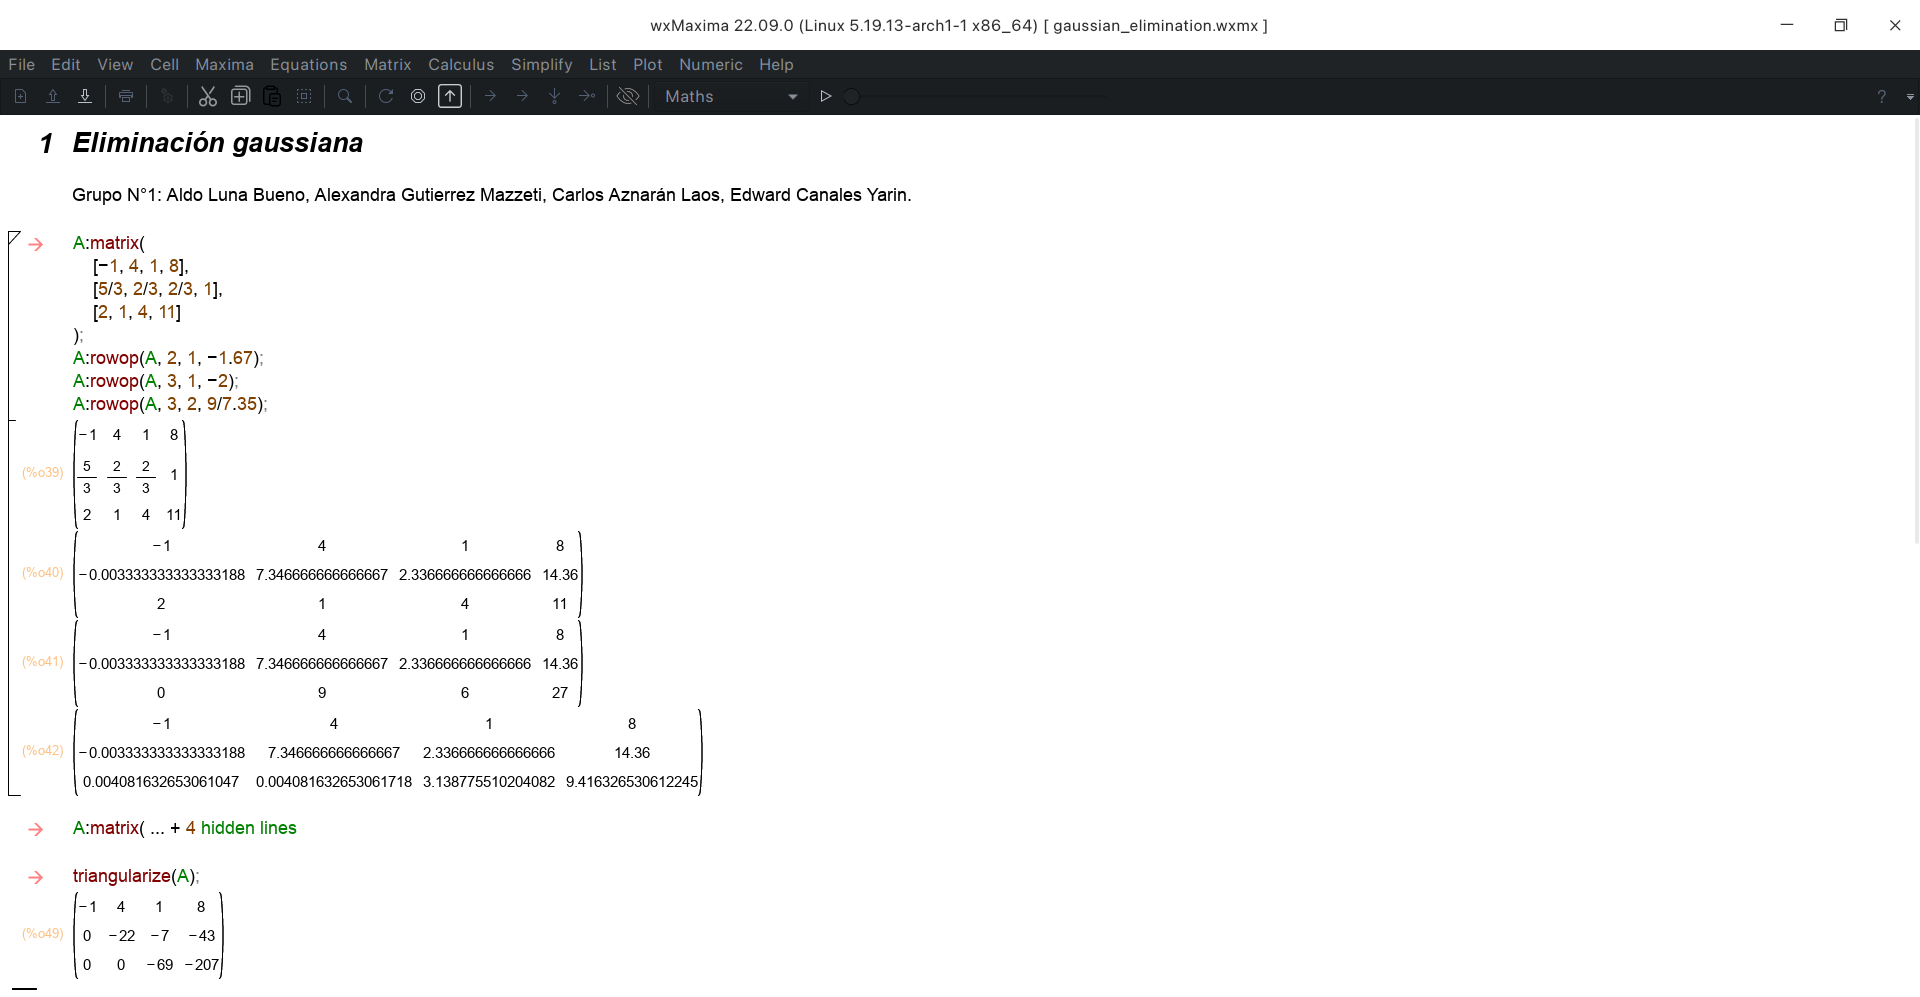
\includegraphics[width=\paperwidth]{gaussian_elimination}}
\begin{frame}[plain]
\end{frame}
}

{
\usebackgroundtemplate{\centering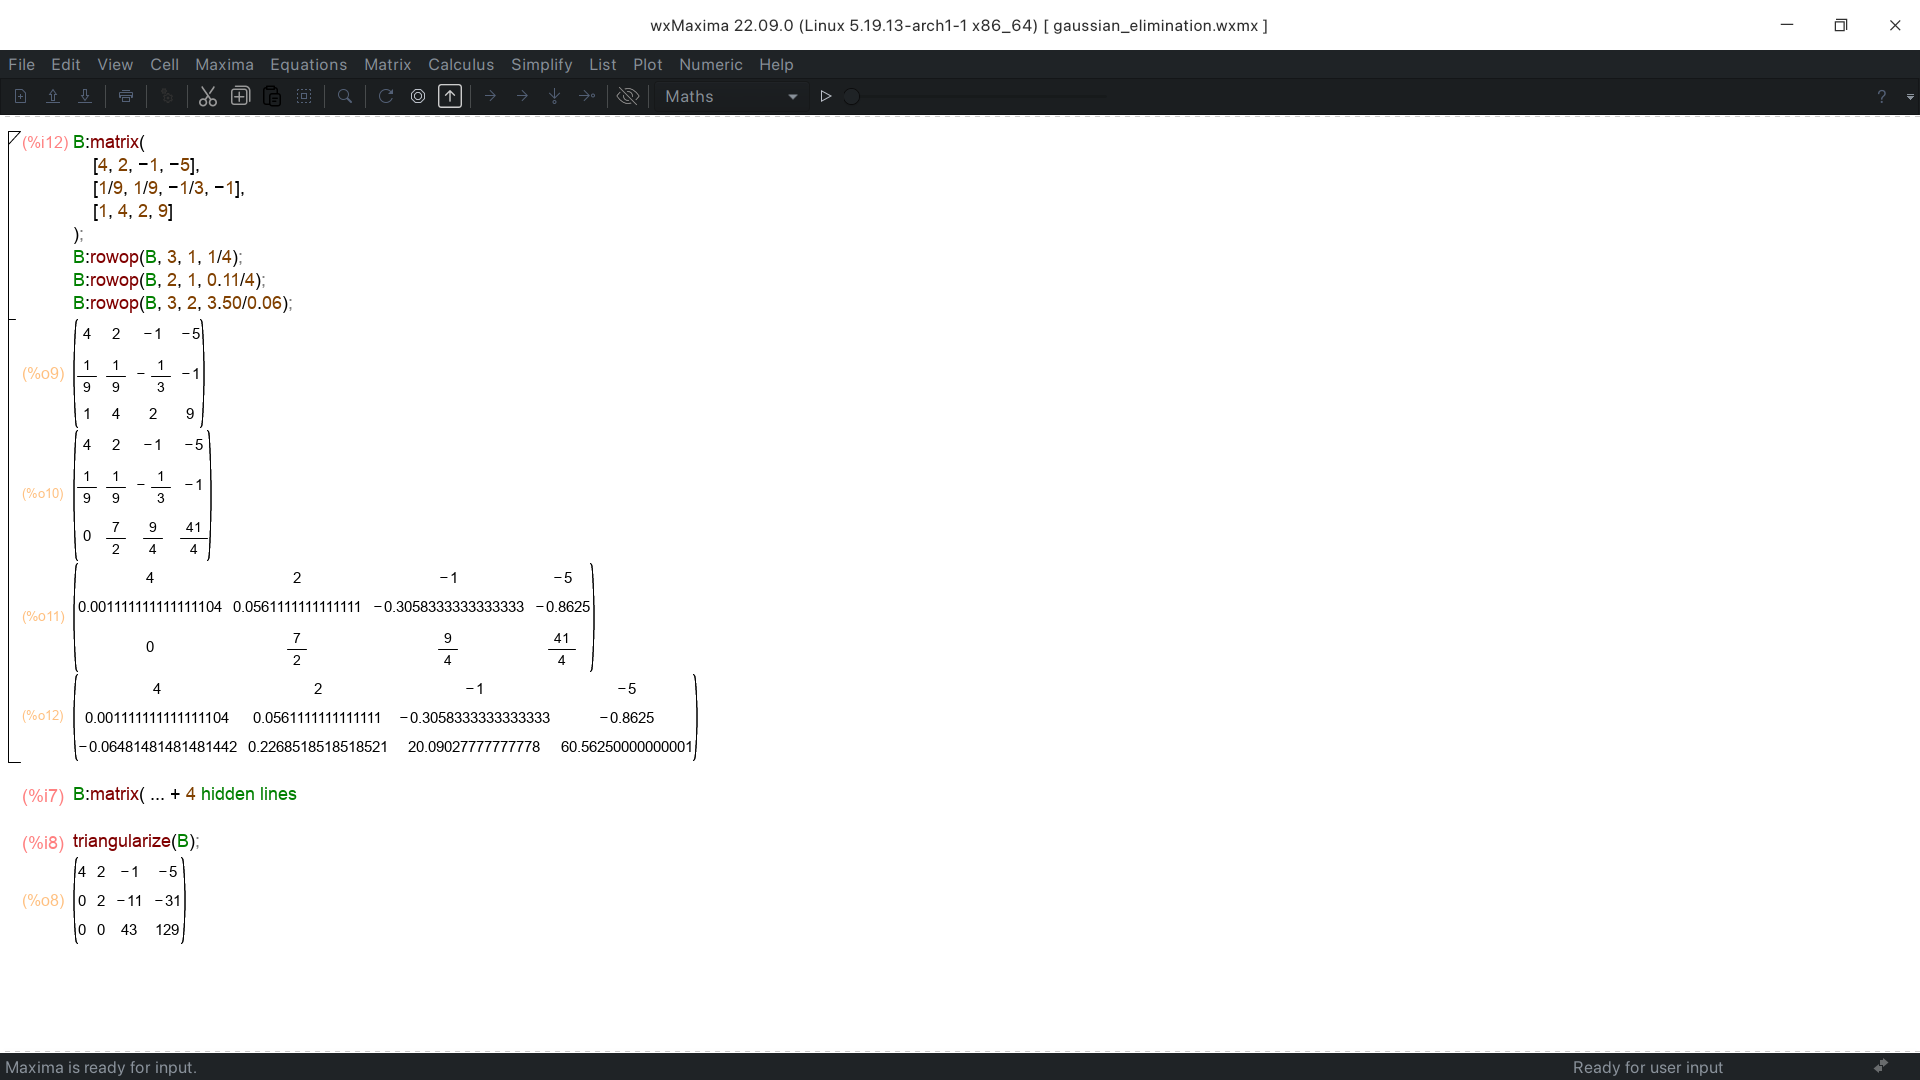
\includegraphics[width=\paperwidth]{gaussian_elimination2}}
\begin{frame}[plain]
\end{frame}
}

% \begin{frame}
% 	\begin{definition}
% 		Sea $A\in\mathbb{C}^{n\times n}$ no singular.
% 		Entonces,
% 		\begin{math}
% 			\operatorname{cond}\left(A\right)=
% 			\left\|A^{-1}\right\|\cdot
% 			\left\|A\right\|
% 		\end{math}
% 		es llamado el \alert{número de condición} de la matriz $A$.
% 	\end{definition}

% 	\begin{lemma}
% 		Suponga que $A\in\mathbb{C}^{n\times n}$ y para alguna norma
% 		matricial natural, $\left\|A\right\|<1$.
% 		Entonces, ${\left(I+A\right)}^{-1}$ existe y
% 		\begin{equation*}
% 			\frac{1}{1+\left\|A\right\|}\leq
% 			\left\|{\left(I+A\right)}^{-1}\right\|\leq
% 			\frac{1}{1-\left\|A\right\|}.
% 		\end{equation*}
% 	\end{lemma}

% 	\begin{proof}
% 		Para $x\in\mathbb{C}^{n}$, $x\neq0$, tenemos
% 		\begin{equation*}
% 			\left\|\left(I+A\right)x\right\|=
% 			\left\|x+Ax\right\|\geq
% 			\left\|x\right\|-\left\|A x\right\|\geq
% 			\left(1-\left\|A\right\|\right)\left\|x\right\|.
% 		\end{equation*}
% 		Esto implica que $\left(I+A\right)x=0$ puede solo cumplirse para
% 		$x=0$,
% 		y así la matriz $\left(I+A\right)$ es no singular.
% 		Más aún, con $C\coloneqq{\left(I+A\right)}^{-1}$, tenemos
% 		\begin{equation*}
% 			1=
% 			\left\|I\right\|=
% 			\left\|\left(I+A\right)C\right\|=
% 			\left\|C+AC\right\|\geq
% 			\left\|C\right\|-\left\|C\right\|\cdot
% 			\left\|A\right\|
% 		\end{equation*}
% 		y análogamente
% 		\begin{math}
% 			1\leq
% 			\left\|C\right\|+
% 			\left\|C\right\|\cdot
% 			\left\|A\right\|
% 		\end{math}.
% 		La combinación de estos hechos conduce a la afirmación.
% 	\end{proof}
% \end{frame}

% \begin{frame}
% 	\begin{lemma}[Lema de perturbación]
% 		Supunga que $A,B\in\mathbb{C}^{n\times n}$ son dos matrices, y
% 		que $A$ es no singular.
% 		Además, suponga que para algunos reales $\alpha$ y $\kappa$,
% 		\begin{math}
% 			\left\|A^{-1}\right\|\leq\alpha
% 		\end{math}
% 		y
% 		\begin{math}
% 			\left\|A^{-1}\right\|\cdot
% 			\left\|B-A\right\|\leq
% 			\kappa<
% 			1,
% 		\end{math}
% 		donde la norma es cualquier norma matricial natural.
% 		Entonces, $B$ es también no singular, y
% 		\begin{math}
% 			\left\|B^{-1}\right\|\leq
% 			\frac{\alpha}{1-\kappa}
% 		\end{math}.
% 	\end{lemma}

% 	\begin{proof}
% 		Dado que
% 		\begin{math}
% 			\left\|A^{-1}(B-A)\right\|\leq
% 			\left\|A^{-1}\right\|\cdot
% 			\|B-A\|<
% 			1,
% 		\end{math}
% 		el lemma implica que $\left(I+A^{-1}(B-A)\right)^{-1}$ existe.
% 		Esto significa que $A^{-1}B$ es también inversible, así $B$ lo
% 		es.
% 		Más aún, el lema da la cota
% 		\begin{equation*}
% 			\left\|B^{-1}\right\|\leq
% 			\left\|B^{-1}A\right\|\cdot
% 			\left\|A^{-1}\right\|\leq
% 			\frac{1}{1-\left\|A^{-1}\right\|\cdot\|B-A\|}\cdot
% 			\alpha\leq
% 			\frac{\alpha}{1-\kappa}.
% 		\end{equation*}
% 	\end{proof}
% \end{frame}

% \begin{frame}
% 	\begin{definition}[La descomposición de valores singulares de una matriz]
% 		Sea $A\in\mathbb{R}^{m\times n}$.
% 		Una descomposición de la forma
% 		\begin{equation*}
% 			A=U\Sigma V^{T},
% 		\end{equation*}
% 		donde $U\in\mathbb{R}^{m\times m}$ y $V\in\mathbb{R}^{n\times n}$
% 		son matrices ortogonales y
% 		\begin{math}
% 			\Sigma=
% 			\left(\sigma_{\mu}\delta_{\mu\nu}\right)
% 			\in\mathbb{R}^{m\times n}
% 		\end{math}
% 		es una matriz diagonal, es llamada una
% 		\alert{decomposition de valores singulares} de $A$.
% 	\end{definition}

% 	\begin{definition}
% 		Suponga que $A\in\mathbb{R}^{m\times n}$ es una matriz con
% 		descomposición de valores singulares $A=U\Sigma V^{T}$.
% 		Entonces,
% 		\begin{math}
% 			\operatorname{cond}_{2}\left(A\right)\coloneqq
% 			\frac{\sigma_{1}}{\sigma_{r}}
% 		\end{math}
% 		es llamado la \alert{condición} de $A$.
% 	\end{definition}
% \end{frame}

% \begin{frame}
% 	Considere el siguiente problema: encuentre $x$ tal que
% 	\begin{equation}\label{problem}
% 		F\left(x,d\right)=0,
% 	\end{equation}
% 	donde $d$ es el conjunto de datos cuya solución depende y $F$ es la
% 	relación funcional entre $x$ y $d$.

% 	\begin{definition}
% 		Para el problema~\eqref{problem} definimos el
% 		\alert{número de condición relativa} como
% 		\begin{equation*}
% 			K\left(d\right)=
% 			\sup\left\{
% 			\frac{
% 				\left\|\delta x\right\|/\left\|x\right\|
% 			}{
% 				\left\|\delta d\right\|/\left\|d\right\|
% 			},
% 			\delta d\neq0,
% 			d+\delta d\in D
% 			\right\}.
% 		\end{equation*}
% 		Siempre que $d=0$ o $x=0$, es necesario introducir el
% 		\alert{número de condición absoluta}, como
% 		\begin{equation*}
% 			K_{\text{abs}}\left(d\right)=
% 			\sup\left\{
% 			\frac{\left\|\delta x\right\|}{\left\|\delta d\right\|},
% 			\delta d\neq0,
% 			d+\delta d\in D
% 			\right\}.
% 		\end{equation*}
% 	\end{definition}
% \end{frame}

% \begin{frame}
% 	Si el problema (2.1) admite una solución unica, entonces existe
% 	necesariamente un mapeo $G$, que llamamos resolvente, entre los
% 	conjuntos de datos y de las soluciones, tal que
% 	\begin{equation*}
% 		x=G\left(d\right),
% 		\text{ esto es }
% 		F\left(G\left(d\right),d\right)=0.
% 	\end{equation*}
% 	Según esta definición, (2.2) da $x+\delta x=G\left(d+\delta d\right)$.
% 	Asumiendo que $G$ es diferenciable en $d$ y denotando formalmente
% 	por $G^{\prime}\left(d\right)$ su derivada con respecto de $d$
% 	(si $G\colon\mathbb{R}^{n}\to\mathbb{R}^{m}, G^{\prime}\left(d\right)$
% 	será la matriz jacobiana de $G$ evaluada en el vector $d$),
% 	la expansión de Taylor de $G$ truncaado en el primer orden asegura que
% 	\begin{equation*}
% 		G
% 		\left(d+\delta d\right)-
% 		G
% 		\left(d\right)=
% 		G^{\prime}
% 		\left(d\right)\delta d+o\left(\left\|\delta d\right\|\right)\quad
% 		\text{ para }\delta d\to 0
% 	\end{equation*}
% 	donde $\left\|\cdot\right\|$ es una norma vectorial adecuada y
% 	$o(\cdot)$ símbolo clásico infinitesimal denotando un término
% 	infinitesimal de orden superior con respecto a su argumento.
% 	Despreciando el infinitesimal de orden superior con respecto a
% 	$\left\|\delta d\right\|$, de (2.4) y (2.5) respectivamente
% 	deducimos que
% 	\begin{equation*}
% 		K\left(d\right)\simeq
% 		\left\|G^{\prime}\left(d\right)\right\|
% 		\frac{\left\|d\right\|}{\left\|G\left(d\right)\right\|},
% 		\quad K_{\text{abs}}\left(d\right)
% 		\simeq\left\|G^{\prime}\left(d\right)\right\|.
% 	\end{equation*}
% \end{frame}

% \begin{frame}
% 	\begin{alertblock}{Ecuaciones no lineales}
% 		Sea $f\colon\mathbb{R}\to\mathbb{R}$ una función de clase $C^{1}$
% 		y considere la ecuación no lineal
% 		\begin{equation*}
% 			F\left(x,d\right)=
% 			f\left(x\right)=
% 			\varphi\left(x\right)-d=
% 			0,
% 		\end{equation*}
% 		donde $\varphi\colon\mathbb{R}\to\mathbb{R}$ es una función
% 		adecuada y $d\in\mathbb{R}$ un dato (posiblemente igual a cero).
% 		El problema está bien definido solo si $\varphi$ es invertible en
% 		una vecindad de $d$: en tal caso, de hecho,
% 		$x=\varphi^{-1}\left(d\right)$ y el resolvente es
% 		$G=\varphi^{-1}$.
% 		Ya que
% 		\begin{math}
% 			{\left(\varphi^{-1}\right)}^{\prime}
% 			\left(d\right)=
% 			{\left[\varphi^{\prime}\left(x\right)\right]}^{-1}
% 		\end{math},
% 		la primera relación en (2.7) da, para $d\neq0$,
% 		\begin{equation*}
% 			K\left(d\right)\simeq
% 			\left|
% 			{\left[{\varphi}^{\prime}\left(x\right)\right]}^{-1}
% 			\right|
% 			\frac{\left|d\right|}{\left|x\right|},
% 		\end{equation*}
% 		mientras si $d=0$ o $x=0$ tenemos
% 		\begin{equation*}
% 			K_{\text{abs}}\left(d\right)\simeq
% 			\left|
% 			{\left[{\varphi}^{\prime}\left(x\right)\right]}^{-1}
% 			\right|.
% 		\end{equation*}
% 	\end{alertblock}
% \end{frame}

\begin{frame}\transblindsvertical
	\frametitle{Referencias}
	%------------------------------------------------------------ 1
	\only<1>{
		\begin{itemize}
			\item Libros
			      \nocite{*}
			      \printbibliography[heading=none,keyword=book]
		\end{itemize}
	}
	%------------------------------------------------------------ 2
	\only<2>{
		\begin{itemize}
			\item Artículos científicos
			      \printbibliography[heading=none,keyword=paper]
		\end{itemize}
	}
	%------------------------------------------------------------ 3
	\only<3>{
		\begin{itemize}
			\item Sitios web
			      \printbibliography[heading=none,keyword=online]
		\end{itemize}
	}
\end{frame}

\end{document}